

\section{Bluetoothkommunikation, Messung und Persistierung} 

Um Messdaten zu erhalten, kommuniziert ApoCo mit den Messsensoren \"uber Bluetooth.
Die eingesetzten Sensoren der Firma BodyTel verwenden f\"ur die \"Ubermittlung der Messdaten 
ein Protokoll, das dem \emph{PDU-Modus} einer SMS entspricht.
PDU steht f\"ur \emph{Protocol Data Unit} und ist eine von drei Spezifikationen, 
welche vom \emph{Europ\"aischen Institut f\"ur Telekommunikationsnormen} (ETSI)\cite{ETSI:01}
zum Standard f\"ur SMS-Nachrichten erkl\"art wurde.
In diesem Protokoll werden AT-Kommandos f\"ur den Verbindungsaufbau eingesetzt 
und anschlie\ss{}end die Messwerte im PDU-Modus \"ubermittelt. 
AT-Kommandos sind ein Befehlssatz, der zum Parametrieren und Konfigurieren von Modems genutzt wird\cite{AT-command:01}.
Mit einem AT-Kommando teilt der Messsensor der Software mit, wenn er im n\"achsten Schritt eine Nachricht \"ubermitteln m\"ochte.
Da jeder Messsensor nur f\"ur eine bestimmte Art von Messung geeignet ist, underscheiden sich die PDUs der einzelnen Ger\"ate.
Nach dem ein Sensor \"uber Bluetooth mit dem Smartphone gekoppelt ist und verwendet werden soll, muss ApoCo 
als Bluetooth-Server auf ankommende Nachrichten h\"oren.\\
Im Gegensatz zu der Bluetoothkommunikation der BodyTel-Ger\"ate wird bei der Verbindung mit der Laborwaage f\"ur das Abwiegen
von Lebensmitteln kein Kommunikationsprotokoll verwendet.
Die Waage kommuniziert \"uber eine RS-232-Schnittstelle direkt ohne die Nachricht zu kodieren.
An dieser Schnittstelle sitzt ein Bluetooth-Dongle und ersetzt ein serielles Kabel.
ApoCo baut eine BluetoothSocket-Verbindung zu der Bluetooth-Dongle Adresse auf.
Die Waage sendet die Messwerte im 8-Bit ASCII-Code. 
Was beim Wiegen an Daten gesendet wird, kann an der Waage parametriert werden.
F\"ur die Kommunikation mit ApoCo wird das gemessene Nettogewicht \"ubertragen.
Direkt nachdem eine Socketverbindung zwischen ApoCo und der Waage aufgebaut ist, 
k\"onnen Daten von der Waage im ASCII-Code empfangen werden.\\


\subsection{Bluetoothkommunikation BodyTel}

In der Abbildung 4.5 wird am Beispiel der K\"orpergewichtsmessung demonstriert,
wie ein Verbindungsaufbau und Datenaustausch zwischen ApoCo und der K\"orperwaage zustande kommt.
Nach dem Start initialisiert die Activity \emph{ActivityBodyweight} den \emph{BluetoothManager} 
und erzeugt ein Objekt vom Typ \emph{WeightTelCreator}.
Anschlie\ss{}end wird die Methode \emph{listenForInquiryConnections()} des \emph{BluetoothManager} gerufen.
Dabei \"ubergibt die Activity der Methode ein Objekt vom Typ Handler und \emph{WeightTelCreator}.
Der Handler ist zust\"andig f\"ur Intraprozesskommunikation zwischen der Activity und einem Thread.
Kommt eine Nachricht \"uber den BluetoothSocket rein, so kann diese nicht direkt an die Activity gegeben werden.
Das kann der Thread nur \"uber den Handler tun.
Der \emph{WeightTelCreator} erzeugt den Thread und gibt eine Referenz auf ihn zur\"uck.
Die Referenz ist eine Schnittstelle vom Typ \emph{AccessableIF}.
\"Uber diese Schnittstelle kann die Activity Nachrichten an den Thread senden.
Daf\"ur gibt es die folgenden Methoden:

\begin{itemize}
 \item writeTo():\\
 \"Uber diese Methode k\"onnen Nachrichten an den Thread gesendet werden.
 Der Thread leitet die Nachrichten \"uber den BluetoothSocket an den Messsensor weiter.
 \item preformStart():\\
 Mit dieser Methode wird der Thread von der Activity gestartet.
 \item cancel();\\
 Mit dieser Methode fordert die Activity den Thread auf sich zu beenden.
\end{itemize}


\begin{figure}[h]
  \centering
  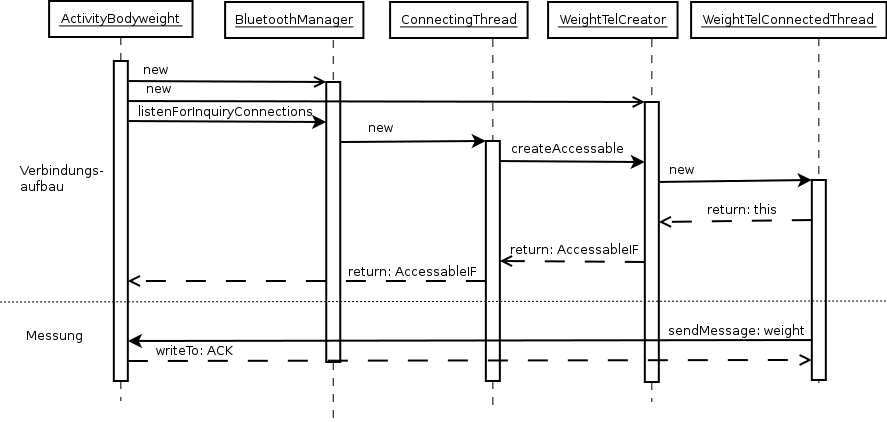
\includegraphics[scale=0.5]{diagramme/kapitel4/sequenzdiagramme/bt_com_aufbau_datasend.png}
  \caption{Sequenzdiagramm f\"ur Bluetoothverbindung und Datenaustausch}
  
\end{figure}

\subsection{Dekodieren einer Messung}

Das Dekodieren einer Messung wird am Beispiel der K\"orpergewichtsmessung erkl\"art.
Um eine Messung zu bekommen, muss zuerst das Protokoll der BodyTel-Ger\"ate erf\"ullt werden.
Der Ablauf dabei sieht folgenderma\ss{}en aus:
\begin{itemize}
 \item Sensor sendet: ATE0\\
 Das ist ein Echo und pr\"uft, ob jemand antwortet.
 \item ApoCo sendet: \textbackslash n \textbackslash r OK \textbackslash n \textbackslash r\\
 Antwort auf das Echo.
 \item Sensor sendet: AT+CMGS=142\\
 Das Kommando vor dem Gleichheitszeichen bedeutet, es wird eine Nachricht gesendet 
 und die Zahl danach ist die L\"ange der SMS.
 \item Sensor sendet: Nachricht als Hexadezimalzahlen.
 \item ApoCo sendet: \textbackslash r \textbackslash n +CMGS\\
 Best\"atigung der Nachricht.
\end{itemize}
Ende der Kommunikation.\\

Ab jetzt muss die Nachricht dekodiert werden. 
Daf\"ur veranschaulicht die Abbildung 4.6 in einem Klassendiagramm, welche Klassen f\"ur diesen Vorgang notwendig sind.

\begin{figure}[h]
  \centering
  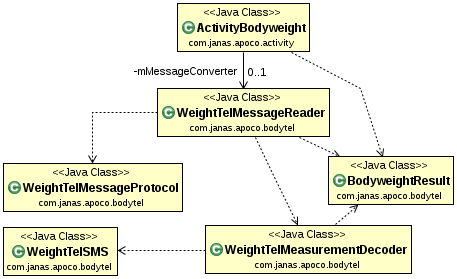
\includegraphics[scale=0.78]{diagramme/kapitel4/uml/weighttel_messagedecode.png}
  \caption{Klassendiagramm f\"ur Dekodieren von Nachrichten}
  
\end{figure}

Zum Einlesen der ankommenden Nachricht benutzt die Klasse \emph{ActivityBodyweight} ein Objekt der 
Klasse \emph{WeightTelMessageReader}.
Die Klasse \emph{WeightTelMessageReader} analysiert  die Nachricht und setzt die einzelnen ankommenden Bl\"ocke in einem St\"uck zusammen.
W\"ahrend der Analyse ordnet die Klasse \emph{WeightTelMessageReader} die richtigen Antwort-Strings zu, 
die an den Sensor zur\"uckgegeben werden.
F\"ur diese Analyse stehen in der Klasse \emph{WeightTelMessageProtocol} die entsprechenden Konstanten bereit.
Wurde die Nachricht zum Ende gelesen, wird die SMS als String an die Klasse \emph{WeightTelMeasurementDecoder} weitergereicht.
Hier wird die Methode \emph{decodeMeasurement()} aufgerufen.
Die Klasse \emph{WeightTelMeasurementDecoder} erzeugt ein Objekt vom Typ \emph{WeightTelSMS} und initialisiert es mit dem SMS-String.
Im Konstruktor der Klasse \emph{WeightTelSMS} wird der SMS-String an entsprechenden Stellen getrennt und in lesbare Werte umgewandelt.
Nach diesem Vorgang erzeugt die Klasse \emph{WeightTelMeasurementDecoder} ein Objekt von Typ \emph{BodyweightResult} und 
initialisiert es mit den Messergebnissen aus dem \emph{WeightTelSMS}-Objekt.
Das \emph{Result}-Objekt wird anschlie\ss{}end an die Activity durchgereicht.
Dieser Vorgang wird durch das Sequenzdiagramm in der Abbildung 4.7 verdeutlicht.\\

\begin{figure}[h]
  \centering
  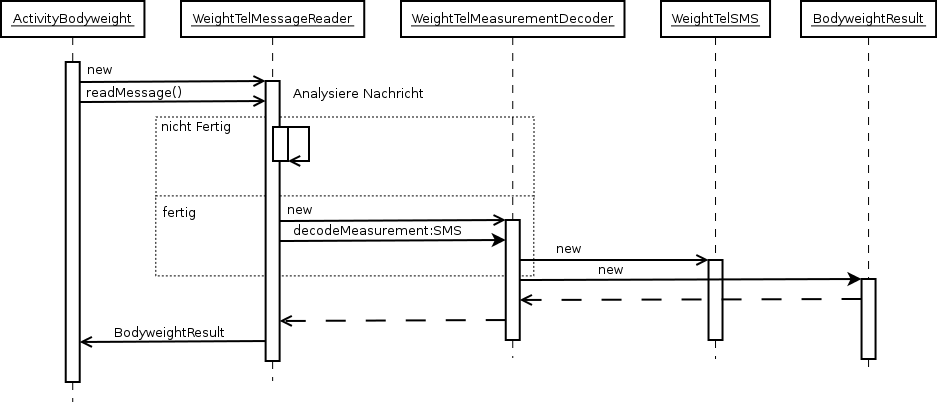
\includegraphics[scale=0.45]{diagramme/kapitel4/sequenzdiagramme/weighttel_messagedecode.png}
  \caption{Sequenzdiagramm f\"ur Dekodieren von Nachrichten}
  
\end{figure}

\subsection{Anzeigen und Speichern der Messwerte}

Nach einer Messung erscheint der neue Messwert ganz oben in einer ListView der Activity und wird anschlie\ss{}end 
in der Datenbank gespeichert.
Das funktioniert folgenderma\ss{}en:
Wenn das \emph{Result}-Objekt nach dem Dekodieren der SMS an die Activity durchgegeben wurde, 
erzeugt der Handler der Activity ein \emph{DTO}-Objekt.
Im Fall der K\"orpergewichtsmessung ist das ein Objekt der Klasse \emph{BodyweightDTO}.
Dieses Objekt wird mit dem \emph{Result}-Objekt initialisiert.
Nun wird aus dem \emph{DTO}-Objekt mit Hilfe der static Methode \emph{\texttt{convertDTO\_to\_MODEL()}} 
der Klasse \emph{BodyweightModel}, ein Objekt
der Klasse \emph{BodyweightModel}  erzeugt und an einen ArrayAdapter zum Anzeigen in der ListView \"ubergeben.
Das \emph{DTO}-Objekt wird durch die Klasse \emph{DBManagerLocal} in der Datenbank gespeichert.
Dieser Vorgang soll durch die Diagramme in den Abbildungen 4.8 und 4.9 nochmals verdeutlicht werden.


\begin{figure}[h]
  \centering
  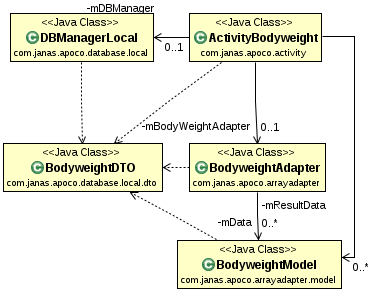
\includegraphics[scale=0.8]{diagramme/kapitel4/uml/show_results_in_lv.png}
  \caption{Klassendiagramm, Visualisierung und Speicherung der Daten}
  
\end{figure}

\begin{figure}[h]
  \centering
  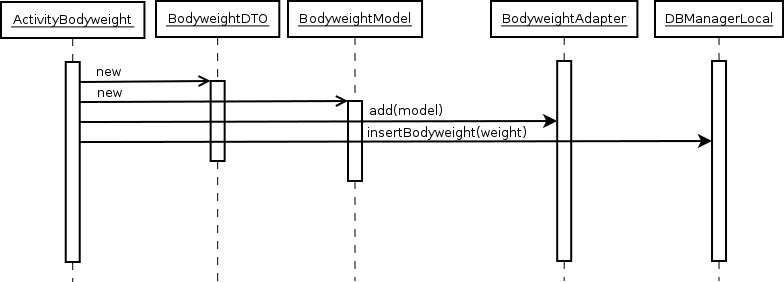
\includegraphics[scale=0.5]{diagramme/kapitel4/sequenzdiagramme/vl_db.png}
  \caption{Sequenzdiagramm, Visualisierung und Speicherung der Daten}
  
\end{figure}